% Options for packages loaded elsewhere
\PassOptionsToPackage{unicode}{hyperref}
\PassOptionsToPackage{hyphens}{url}
%
\documentclass[
]{article}
\usepackage{amsmath,amssymb}
\usepackage{iftex}
\ifPDFTeX
  \usepackage[T1]{fontenc}
  \usepackage[utf8]{inputenc}
  \usepackage{textcomp} % provide euro and other symbols
\else % if luatex or xetex
  \usepackage{unicode-math} % this also loads fontspec
  \defaultfontfeatures{Scale=MatchLowercase}
  \defaultfontfeatures[\rmfamily]{Ligatures=TeX,Scale=1}
\fi
\usepackage{lmodern}
\ifPDFTeX\else
  % xetex/luatex font selection
\fi
% Use upquote if available, for straight quotes in verbatim environments
\IfFileExists{upquote.sty}{\usepackage{upquote}}{}
\IfFileExists{microtype.sty}{% use microtype if available
  \usepackage[]{microtype}
  \UseMicrotypeSet[protrusion]{basicmath} % disable protrusion for tt fonts
}{}
\makeatletter
\@ifundefined{KOMAClassName}{% if non-KOMA class
  \IfFileExists{parskip.sty}{%
    \usepackage{parskip}
  }{% else
    \setlength{\parindent}{0pt}
    \setlength{\parskip}{6pt plus 2pt minus 1pt}}
}{% if KOMA class
  \KOMAoptions{parskip=half}}
\makeatother
\usepackage{xcolor}
\usepackage[margin=1in]{geometry}
\usepackage{color}
\usepackage{fancyvrb}
\newcommand{\VerbBar}{|}
\newcommand{\VERB}{\Verb[commandchars=\\\{\}]}
\DefineVerbatimEnvironment{Highlighting}{Verbatim}{commandchars=\\\{\}}
% Add ',fontsize=\small' for more characters per line
\usepackage{framed}
\definecolor{shadecolor}{RGB}{248,248,248}
\newenvironment{Shaded}{\begin{snugshade}}{\end{snugshade}}
\newcommand{\AlertTok}[1]{\textcolor[rgb]{0.94,0.16,0.16}{#1}}
\newcommand{\AnnotationTok}[1]{\textcolor[rgb]{0.56,0.35,0.01}{\textbf{\textit{#1}}}}
\newcommand{\AttributeTok}[1]{\textcolor[rgb]{0.13,0.29,0.53}{#1}}
\newcommand{\BaseNTok}[1]{\textcolor[rgb]{0.00,0.00,0.81}{#1}}
\newcommand{\BuiltInTok}[1]{#1}
\newcommand{\CharTok}[1]{\textcolor[rgb]{0.31,0.60,0.02}{#1}}
\newcommand{\CommentTok}[1]{\textcolor[rgb]{0.56,0.35,0.01}{\textit{#1}}}
\newcommand{\CommentVarTok}[1]{\textcolor[rgb]{0.56,0.35,0.01}{\textbf{\textit{#1}}}}
\newcommand{\ConstantTok}[1]{\textcolor[rgb]{0.56,0.35,0.01}{#1}}
\newcommand{\ControlFlowTok}[1]{\textcolor[rgb]{0.13,0.29,0.53}{\textbf{#1}}}
\newcommand{\DataTypeTok}[1]{\textcolor[rgb]{0.13,0.29,0.53}{#1}}
\newcommand{\DecValTok}[1]{\textcolor[rgb]{0.00,0.00,0.81}{#1}}
\newcommand{\DocumentationTok}[1]{\textcolor[rgb]{0.56,0.35,0.01}{\textbf{\textit{#1}}}}
\newcommand{\ErrorTok}[1]{\textcolor[rgb]{0.64,0.00,0.00}{\textbf{#1}}}
\newcommand{\ExtensionTok}[1]{#1}
\newcommand{\FloatTok}[1]{\textcolor[rgb]{0.00,0.00,0.81}{#1}}
\newcommand{\FunctionTok}[1]{\textcolor[rgb]{0.13,0.29,0.53}{\textbf{#1}}}
\newcommand{\ImportTok}[1]{#1}
\newcommand{\InformationTok}[1]{\textcolor[rgb]{0.56,0.35,0.01}{\textbf{\textit{#1}}}}
\newcommand{\KeywordTok}[1]{\textcolor[rgb]{0.13,0.29,0.53}{\textbf{#1}}}
\newcommand{\NormalTok}[1]{#1}
\newcommand{\OperatorTok}[1]{\textcolor[rgb]{0.81,0.36,0.00}{\textbf{#1}}}
\newcommand{\OtherTok}[1]{\textcolor[rgb]{0.56,0.35,0.01}{#1}}
\newcommand{\PreprocessorTok}[1]{\textcolor[rgb]{0.56,0.35,0.01}{\textit{#1}}}
\newcommand{\RegionMarkerTok}[1]{#1}
\newcommand{\SpecialCharTok}[1]{\textcolor[rgb]{0.81,0.36,0.00}{\textbf{#1}}}
\newcommand{\SpecialStringTok}[1]{\textcolor[rgb]{0.31,0.60,0.02}{#1}}
\newcommand{\StringTok}[1]{\textcolor[rgb]{0.31,0.60,0.02}{#1}}
\newcommand{\VariableTok}[1]{\textcolor[rgb]{0.00,0.00,0.00}{#1}}
\newcommand{\VerbatimStringTok}[1]{\textcolor[rgb]{0.31,0.60,0.02}{#1}}
\newcommand{\WarningTok}[1]{\textcolor[rgb]{0.56,0.35,0.01}{\textbf{\textit{#1}}}}
\usepackage{graphicx}
\makeatletter
\def\maxwidth{\ifdim\Gin@nat@width>\linewidth\linewidth\else\Gin@nat@width\fi}
\def\maxheight{\ifdim\Gin@nat@height>\textheight\textheight\else\Gin@nat@height\fi}
\makeatother
% Scale images if necessary, so that they will not overflow the page
% margins by default, and it is still possible to overwrite the defaults
% using explicit options in \includegraphics[width, height, ...]{}
\setkeys{Gin}{width=\maxwidth,height=\maxheight,keepaspectratio}
% Set default figure placement to htbp
\makeatletter
\def\fps@figure{htbp}
\makeatother
\setlength{\emergencystretch}{3em} % prevent overfull lines
\providecommand{\tightlist}{%
  \setlength{\itemsep}{0pt}\setlength{\parskip}{0pt}}
\setcounter{secnumdepth}{-\maxdimen} % remove section numbering
\usepackage{multirow}
\usepackage{multicol}
\usepackage{colortbl}
\usepackage{hhline}
\newlength\Oldarrayrulewidth
\newlength\Oldtabcolsep
\usepackage{longtable}
\usepackage{array}
\usepackage{hyperref}
\usepackage{float}
\usepackage{wrapfig}
\ifLuaTeX
  \usepackage{selnolig}  % disable illegal ligatures
\fi
\usepackage{bookmark}
\IfFileExists{xurl.sty}{\usepackage{xurl}}{} % add URL line breaks if available
\urlstyle{same}
\hypersetup{
  pdftitle={STAT462 Assignment 1},
  pdfauthor={Simon Clark (XXXXXXXX); David Ewing (82171165); Xia Yu (62380486)},
  hidelinks,
  pdfcreator={LaTeX via pandoc}}

\title{STAT462 Assignment 1}
\author{Simon Clark (XXXXXXXX) \and David Ewing (82171165) \and Xia Yu
(62380486)}
\date{2025-03-11}

\begin{document}
\maketitle

\section{Load all Data}\label{load-all-data}

\section{Braking Distance}\label{braking-distance}

In this question, do not use the \texttt{lm} function or a module that
provides an implementation of k-NN. You are allowed to use elementary
statistical objects like mean, variance, etc.

We will be predicting the distance that a car takes to stop when driving
at a certain speed. The dataset is from 1930, so it might be slightly
outdated. Units are miles per hour (speed) and feet (distance).

\subsection{Data Preparation}\label{data-preparation}

\begin{Shaded}
\begin{Highlighting}[]
\CommentTok{\# Load and preprocess dataset}
\end{Highlighting}
\end{Shaded}

\subsection{Linear Regression (Without
lm)}\label{linear-regression-without-lm}

\begin{Shaded}
\begin{Highlighting}[]
\CommentTok{\# Compute slope and intercept for simple linear regression}
\end{Highlighting}
\end{Shaded}

Using the linear regression model, predict the braking distance for a
car going at 30 km/h and include an 80\% prediction interval.

\begin{Shaded}
\begin{Highlighting}[]
\CommentTok{\# Prediction for 30 km/h}
\end{Highlighting}
\end{Shaded}

\subsection{k-NN Model}\label{k-nn-model}

\begin{Shaded}
\begin{Highlighting}[]
\CommentTok{\# Fit and predict using k{-}NN model}
\end{Highlighting}
\end{Shaded}

\section{Filipino Household Income}\label{filipino-household-income}

\begin{center}\rule{0.5\linewidth}{0.5pt}\end{center}

\subsection{Data Preparation}\label{data-preparation-1}

\begin{Shaded}
\begin{Highlighting}[]
\CommentTok{\# Ensure dplyr is loaded}
\CommentTok{\# library(dplyr)}
\CommentTok{\# library(skimr)}
\CommentTok{\# library(flextable)  \# Ensure flextable is loaded}
\end{Highlighting}
\end{Shaded}

\begin{Shaded}
\begin{Highlighting}[]
    \CommentTok{\# Loads the income.csv dataset from a zipped file located at zip\_path}
\NormalTok{zip\_path }\OtherTok{\textless{}{-}} \StringTok{"../data/datasets.zip"}
\ControlFlowTok{if}\NormalTok{ (}\FunctionTok{file.exists}\NormalTok{(zip\_path)) \{}
\NormalTok{income\_dataset }\OtherTok{\textless{}{-}} \FunctionTok{read.csv}\NormalTok{(}\FunctionTok{unz}\NormalTok{(zip\_path, }\StringTok{"income.csv"}\NormalTok{))}
\NormalTok{\} }\ControlFlowTok{else}\NormalTok{ \{}
  \FunctionTok{stop}\NormalTok{(}\StringTok{"The zip file does not exist at the given path."}\NormalTok{)}
\NormalTok{\}}

\CommentTok{\# Uses the skim function from the skimr package to generate a summary of the dataset and then selects the skim\_variable and n\_missing columns, which likely represent variable names and the count of missing values, respectively.}
\NormalTok{skimp }\OtherTok{\textless{}{-}} \FunctionTok{skim}\NormalTok{(income\_dataset) }\SpecialCharTok{|\textgreater{}}
  \FunctionTok{select}\NormalTok{(skim\_variable, n\_missing)}

\CommentTok{\# Prints the summary (stored in the skimp object).}
\NormalTok{skimp}
\end{Highlighting}
\end{Shaded}

\begin{verbatim}
## # A tibble: 60 x 2
##    skim_variable                            n_missing
##    <chr>                                        <int>
##  1 Region                                           0
##  2 Main.Source.of.Income                            0
##  3 Household.Head.Sex                               0
##  4 Household.Head.Marital.Status                    0
##  5 Household.Head.Highest.Grade.Completed           0
##  6 Household.Head.Job.or.Business.Indicator         0
##  7 Household.Head.Occupation                     7536
##  8 Household.Head.Class.of.Worker                7536
##  9 Type.of.Household                                0
## 10 Type.of.Building.House                           0
## # i 50 more rows
\end{verbatim}

\begin{Shaded}
\begin{Highlighting}[]
\CommentTok{\# Extracts two specific columns (Total.Household.Income and Members.with.age.5...17.years.old) from the dataset and renames them to income and children, respectively.}
\NormalTok{income }\OtherTok{\textless{}{-}}\NormalTok{ income\_dataset}\SpecialCharTok{$}\NormalTok{Total.Household.Income}
\NormalTok{children }\OtherTok{\textless{}{-}}\NormalTok{ income\_dataset}\SpecialCharTok{$}\NormalTok{Members.with.age.}\DecValTok{5}\NormalTok{...}\FloatTok{17.}\NormalTok{years.old}
\end{Highlighting}
\end{Shaded}

\subsubsection{Data Initial Summary}\label{data-initial-summary}

\begin{Shaded}
\begin{Highlighting}[]
\CommentTok{\# summaries of variables}
\FunctionTok{cat}\NormalTok{(}\StringTok{"}\SpecialCharTok{\textbackslash{}n}\StringTok{Summary of Household Income:}\SpecialCharTok{\textbackslash{}n}\StringTok{"}\NormalTok{, }
    \FunctionTok{paste}\NormalTok{(}\FunctionTok{names}\NormalTok{(}\FunctionTok{summary}\NormalTok{(income)), }\FunctionTok{summary}\NormalTok{(income), }\AttributeTok{sep =} \StringTok{" = "}\NormalTok{, }\AttributeTok{collapse =} \StringTok{"}\SpecialCharTok{\textbackslash{}n}\StringTok{"}\NormalTok{), }\StringTok{"}\SpecialCharTok{\textbackslash{}n\textbackslash{}n}\StringTok{"}\NormalTok{)}
\end{Highlighting}
\end{Shaded}

\begin{verbatim}
## 
## Summary of Household Income:
##  Min. = 11285
## 1st Qu. = 104895
## Median = 164079.5
## Mean = 247555.584801656
## 3rd Qu. = 291138.5
## Max. = 11815988
\end{verbatim}

\begin{Shaded}
\begin{Highlighting}[]
\FunctionTok{cat}\NormalTok{(}\StringTok{"Summary of Number of Children:}\SpecialCharTok{\textbackslash{}n}\StringTok{"}\NormalTok{, }
    \FunctionTok{paste}\NormalTok{(}\FunctionTok{names}\NormalTok{(}\FunctionTok{summary}\NormalTok{(children)), }\FunctionTok{summary}\NormalTok{(children), }\AttributeTok{sep =} \StringTok{" = "}\NormalTok{, }\AttributeTok{collapse =} \StringTok{"}\SpecialCharTok{\textbackslash{}n}\StringTok{"}\NormalTok{), }\StringTok{"}\SpecialCharTok{\textbackslash{}n}\StringTok{"}\NormalTok{)}
\end{Highlighting}
\end{Shaded}

\begin{verbatim}
## Summary of Number of Children:
##  Min. = 0
## 1st Qu. = 0
## Median = 1
## Mean = 1.36257943385326
## 3rd Qu. = 2
## Max. = 8
\end{verbatim}

\subsubsection{Scatter Plot Of Target
Data}\label{scatter-plot-of-target-data}

\begin{Shaded}
\begin{Highlighting}[]
\CommentTok{\# Scatter plot of income vs. children}
\FunctionTok{plot}\NormalTok{(children, income}\SpecialCharTok{/}\DecValTok{10000}\NormalTok{, }\AttributeTok{xlab =} \StringTok{"Number of Children"}\NormalTok{, }\AttributeTok{ylab =} \StringTok{"Household Income (in 10 Thousands)"}\NormalTok{, }\AttributeTok{main =} \StringTok{"Income vs. Children"}\NormalTok{)}
\end{Highlighting}
\end{Shaded}

\includegraphics{20250310-STAT462A1-Framework_files/figure-latex/unnamed-chunk-20-1.pdf}

\subsection{Linear Regression}\label{linear-regression}

\subsubsection{Training Set And Testing Set
Preparation}\label{training-set-and-testing-set-preparation}

\begin{Shaded}
\begin{Highlighting}[]
\CommentTok{\# set a seed for reproducibility and reduce RAM pressure.}
\FunctionTok{set.seed}\NormalTok{(}\DecValTok{888}\NormalTok{)  }
\CommentTok{\# combine income and children into a data frame}
\NormalTok{data }\OtherTok{\textless{}{-}} \FunctionTok{data.frame}\NormalTok{(}\AttributeTok{income =}\NormalTok{ income, }\AttributeTok{children =}\NormalTok{ children)}
\CommentTok{\# Subset the data into training and test sets}

\CommentTok{\# Generate a random sample of row indices for training set (80\% of the data)}
\NormalTok{train\_indices }\OtherTok{\textless{}{-}} \FunctionTok{sample}\NormalTok{(}\DecValTok{1}\SpecialCharTok{:}\FunctionTok{nrow}\NormalTok{(data), }\AttributeTok{size =} \FloatTok{0.8} \SpecialCharTok{*} \FunctionTok{nrow}\NormalTok{(data))}
\CommentTok{\# Subset the data into training and test sets}
\NormalTok{train\_data }\OtherTok{\textless{}{-}}\NormalTok{ data[train\_indices, ]}
\NormalTok{test\_data }\OtherTok{\textless{}{-}}\NormalTok{ data[}\SpecialCharTok{{-}}\NormalTok{train\_indices, ]  }\CommentTok{\# Use the remaining data for testing}
\end{Highlighting}
\end{Shaded}

\subsubsection{Model Training}\label{model-training}

\begin{Shaded}
\begin{Highlighting}[]
\CommentTok{\# fit a linear regression model}
\NormalTok{model }\OtherTok{\textless{}{-}} \FunctionTok{lm}\NormalTok{(income }\SpecialCharTok{\textasciitilde{}}\NormalTok{ children, }\AttributeTok{data =}\NormalTok{ train\_data)}

\CommentTok{\# print the summary of the model}
\FunctionTok{summary}\NormalTok{(model)}
\end{Highlighting}
\end{Shaded}

\begin{verbatim}
## 
## Call:
## lm(formula = income ~ children, data = train_data)
## 
## Residuals:
##      Min       1Q   Median       3Q      Max 
##  -251450  -140741   -79204    45428 11553253 
## 
## Coefficients:
##             Estimate Std. Error t value Pr(>|t|)    
## (Intercept)   262735       2181  120.45   <2e-16 ***
## children      -11256       1112  -10.12   <2e-16 ***
## ---
## Signif. codes:  0 '***' 0.001 '**' 0.01 '*' 0.05 '.' 0.1 ' ' 1
## 
## Residual standard error: 285600 on 33233 degrees of freedom
## Multiple R-squared:  0.003072,   Adjusted R-squared:  0.003042 
## F-statistic: 102.4 on 1 and 33233 DF,  p-value: < 2.2e-16
\end{verbatim}

\subsubsection{Model Explanation}\label{model-explanation}

\textbf{\emph{3.a What is the specific form of the affine-linear model,
i.e.~what are b0 and b1?}}

\begin{itemize}
\item
  The affine-linear model or SLR model (simple linear regression model)
  has the general form:
  \(\text{income} = b_0 + b_1 \cdot \text{children}\)
\item
  \(b_0\) is the \textbf{intercept,} telling the predicted income when
  children = 0. Our model's \(b_0= 262735\)
\item
  \(b_1\) is the \textbf{slope,} representing how income changes per
  additional child. Our model's \(b_1= -11256\)
\item
  So the specific form of our SLR model is:
  \(\text{income} = 262735 −11256 \cdot \text{children}\)
\end{itemize}

\textbf{\emph{3.b.1 What is the predicted mean income of a household
with}} \(𝑛\) \textbf{\emph{children, for}} \(n \in \{0,1,…,8\}\)
\textbf{\emph{?}}

\begin{Shaded}
\begin{Highlighting}[]
\CommentTok{\# Define variables}
\NormalTok{n }\OtherTok{\textless{}{-}} \DecValTok{0}\SpecialCharTok{:}\DecValTok{8}  \CommentTok{\# n is defined as a vector}
\NormalTok{b\_0 }\OtherTok{\textless{}{-}} \DecValTok{262735}
\NormalTok{b\_1 }\OtherTok{\textless{}{-}} \SpecialCharTok{{-}}\DecValTok{11256}

\CommentTok{\# Predict income based on the model}
\NormalTok{predict\_income\_n }\OtherTok{\textless{}{-}}\NormalTok{ b\_0 }\SpecialCharTok{+}\NormalTok{ b\_1 }\SpecialCharTok{*}\NormalTok{ n}
\end{Highlighting}
\end{Shaded}

\textbf{\emph{3.b.2 What are the associated 90\% prediction intervals
(PI)?}}

\(\text{RSE} =\) summary(model)\$sigma

\(\tau = t_\alpha/2 \cdot \text{Residual Standard Error}\)

\(\text{prediction intervals} = \hat{y} \pm \tau\)

\(\text{lower bound} = \hat{y} - \tau\)

\(\text{upper bound} = \hat{y}+\tau\)

\begin{Shaded}
\begin{Highlighting}[]
\CommentTok{\# Compute true mean income for each n from train\_data}
\NormalTok{true\_mean\_income\_n }\OtherTok{\textless{}{-}} \FunctionTok{tapply}\NormalTok{(train\_data}\SpecialCharTok{$}\NormalTok{income, train\_data}\SpecialCharTok{$}\NormalTok{children, mean)}

\CommentTok{\# Get residual standard error from model summary}
\NormalTok{residual\_se }\OtherTok{\textless{}{-}} \FunctionTok{summary}\NormalTok{(model)}\SpecialCharTok{$}\NormalTok{sigma  }\CommentTok{\# Residual standard error}

\CommentTok{\# Find critical value for 90\% prediction interval}
\NormalTok{alpha }\OtherTok{\textless{}{-}} \FloatTok{0.1}
\NormalTok{t\_crit }\OtherTok{\textless{}{-}} \FunctionTok{qt}\NormalTok{(}\DecValTok{1} \SpecialCharTok{{-}}\NormalTok{ alpha}\SpecialCharTok{/}\DecValTok{2}\NormalTok{, }\AttributeTok{df =} \FunctionTok{summary}\NormalTok{(model)}\SpecialCharTok{$}\NormalTok{df[}\DecValTok{2}\NormalTok{])  }\CommentTok{\# Two{-}tailed t{-}value}

\CommentTok{\# Compute the 90\% prediction interval bounds}
\NormalTok{lower\_bound }\OtherTok{\textless{}{-}}\NormalTok{ predict\_income\_n }\SpecialCharTok{{-}}\NormalTok{ t\_crit }\SpecialCharTok{*}\NormalTok{ residual\_se}
\NormalTok{upper\_bound }\OtherTok{\textless{}{-}}\NormalTok{ predict\_income\_n }\SpecialCharTok{+}\NormalTok{ t\_crit }\SpecialCharTok{*}\NormalTok{ residual\_se}
\end{Highlighting}
\end{Shaded}

\textbf{\emph{3.b.3 Summarize all of above infomation in a table.}}

\begin{Shaded}
\begin{Highlighting}[]
\CommentTok{\# Create a data frame}
\NormalTok{test\_results }\OtherTok{\textless{}{-}} \FunctionTok{data.frame}\NormalTok{(}
  \AttributeTok{n =}\NormalTok{ n, }
  \AttributeTok{train\_pred =}\NormalTok{ predict\_income\_n, }
  \AttributeTok{true\_mean\_income\_n =}\NormalTok{ true\_mean\_income\_n[}\FunctionTok{as.character}\NormalTok{(n)],}
  \AttributeTok{lower\_90 =}\NormalTok{ lower\_bound, }
  \AttributeTok{upper\_90 =}\NormalTok{ upper\_bound}
\NormalTok{)}

\CommentTok{\# Create a flextable with custom headers}
\FunctionTok{set\_flextable\_defaults}\NormalTok{(}
    \AttributeTok{font.size =} \DecValTok{8}\NormalTok{, }
    \AttributeTok{theme\_fun =}\NormalTok{ theme\_vanilla,}
    \AttributeTok{padding =} \DecValTok{6}\NormalTok{,}
    \AttributeTok{background.color =} \StringTok{"\#EFEFEF"}\NormalTok{)}
\NormalTok{ft\_test }\OtherTok{\textless{}{-}} \FunctionTok{flextable}\NormalTok{(test\_results) }\SpecialCharTok{|\textgreater{}}
  \FunctionTok{set\_header\_labels}\NormalTok{(}
    \AttributeTok{n =} \StringTok{"Number of Children"}\NormalTok{,}
    \AttributeTok{true\_mean\_income\_n =} \StringTok{"Actual Average Income (with train\_data)"}\NormalTok{,}
    \AttributeTok{train\_pred =} \StringTok{"Predicted Income (with train\_data)"}\NormalTok{,}
    \AttributeTok{lower\_90 =} \StringTok{"Lower Bound (90\% PI)"}\NormalTok{,}
    \AttributeTok{upper\_90 =} \StringTok{"Upper Bound (90\% PI)"}
\NormalTok{  ) }\SpecialCharTok{|\textgreater{}}
\FunctionTok{autofit}\NormalTok{()  }\CommentTok{\# Adjust column sizes automatically}

  
\CommentTok{\# Print the table}
\NormalTok{ft\_test}
\end{Highlighting}
\end{Shaded}

\begin{verbatim}
## Warning: fonts used in `flextable` are ignored because the `pdflatex` engine is
## used and not `xelatex` or `lualatex`. You can avoid this warning by using the
## `set_flextable_defaults(fonts_ignore=TRUE)` command or use a compatible engine
## by defining `latex_engine: xelatex` in the YAML header of the R Markdown
## document.
\end{verbatim}

\global\setlength{\Oldarrayrulewidth}{\arrayrulewidth}

\global\setlength{\Oldtabcolsep}{\tabcolsep}

\setlength{\tabcolsep}{2pt}

\renewcommand*{\arraystretch}{1.5}



\providecommand{\ascline}[3]{\noalign{\global\arrayrulewidth #1}\arrayrulecolor[HTML]{#2}\cline{#3}}

\begin{longtable}[c]{|p{1.36in}|p{2.14in}|p{2.44in}|p{1.50in}|p{1.49in}}



\hhline{>{\arrayrulecolor[HTML]{666666}\global\arrayrulewidth=1.5pt}->{\arrayrulecolor[HTML]{666666}\global\arrayrulewidth=1.5pt}->{\arrayrulecolor[HTML]{666666}\global\arrayrulewidth=1.5pt}->{\arrayrulecolor[HTML]{666666}\global\arrayrulewidth=1.5pt}->{\arrayrulecolor[HTML]{666666}\global\arrayrulewidth=1.5pt}-}

\multicolumn{1}{>{\cellcolor[HTML]{EFEFEF}\raggedleft}m{\dimexpr 1.36in+0\tabcolsep}}{\textcolor[HTML]{000000}{\fontsize{8}{8}\selectfont{\textbf{Number\ of\ Children}}}} & \multicolumn{1}{>{\cellcolor[HTML]{EFEFEF}\raggedleft}m{\dimexpr 2.14in+0\tabcolsep}}{\textcolor[HTML]{000000}{\fontsize{8}{8}\selectfont{\textbf{Predicted\ Income\ (with\ train\_data)}}}} & \multicolumn{1}{>{\cellcolor[HTML]{EFEFEF}\raggedleft}m{\dimexpr 2.44in+0\tabcolsep}}{\textcolor[HTML]{000000}{\fontsize{8}{8}\selectfont{\textbf{Actual\ Average\ Income\ (with\ train\_data)}}}} & \multicolumn{1}{>{\cellcolor[HTML]{EFEFEF}\raggedleft}m{\dimexpr 1.5in+0\tabcolsep}}{\textcolor[HTML]{000000}{\fontsize{8}{8}\selectfont{\textbf{Lower\ Bound\ (90\%\ PI)}}}} & \multicolumn{1}{>{\cellcolor[HTML]{EFEFEF}\raggedleft}m{\dimexpr 1.49in+0\tabcolsep}}{\textcolor[HTML]{000000}{\fontsize{8}{8}\selectfont{\textbf{Upper\ Bound\ (90\%\ PI)}}}} \\

\noalign{\global\arrayrulewidth 0pt}\arrayrulecolor[HTML]{000000}

\hhline{>{\arrayrulecolor[HTML]{666666}\global\arrayrulewidth=1.5pt}->{\arrayrulecolor[HTML]{666666}\global\arrayrulewidth=1.5pt}->{\arrayrulecolor[HTML]{666666}\global\arrayrulewidth=1.5pt}->{\arrayrulecolor[HTML]{666666}\global\arrayrulewidth=1.5pt}->{\arrayrulecolor[HTML]{666666}\global\arrayrulewidth=1.5pt}-}\endfirsthead 

\hhline{>{\arrayrulecolor[HTML]{666666}\global\arrayrulewidth=1.5pt}->{\arrayrulecolor[HTML]{666666}\global\arrayrulewidth=1.5pt}->{\arrayrulecolor[HTML]{666666}\global\arrayrulewidth=1.5pt}->{\arrayrulecolor[HTML]{666666}\global\arrayrulewidth=1.5pt}->{\arrayrulecolor[HTML]{666666}\global\arrayrulewidth=1.5pt}-}

\multicolumn{1}{>{\cellcolor[HTML]{EFEFEF}\raggedleft}m{\dimexpr 1.36in+0\tabcolsep}}{\textcolor[HTML]{000000}{\fontsize{8}{8}\selectfont{\textbf{Number\ of\ Children}}}} & \multicolumn{1}{>{\cellcolor[HTML]{EFEFEF}\raggedleft}m{\dimexpr 2.14in+0\tabcolsep}}{\textcolor[HTML]{000000}{\fontsize{8}{8}\selectfont{\textbf{Predicted\ Income\ (with\ train\_data)}}}} & \multicolumn{1}{>{\cellcolor[HTML]{EFEFEF}\raggedleft}m{\dimexpr 2.44in+0\tabcolsep}}{\textcolor[HTML]{000000}{\fontsize{8}{8}\selectfont{\textbf{Actual\ Average\ Income\ (with\ train\_data)}}}} & \multicolumn{1}{>{\cellcolor[HTML]{EFEFEF}\raggedleft}m{\dimexpr 1.5in+0\tabcolsep}}{\textcolor[HTML]{000000}{\fontsize{8}{8}\selectfont{\textbf{Lower\ Bound\ (90\%\ PI)}}}} & \multicolumn{1}{>{\cellcolor[HTML]{EFEFEF}\raggedleft}m{\dimexpr 1.49in+0\tabcolsep}}{\textcolor[HTML]{000000}{\fontsize{8}{8}\selectfont{\textbf{Upper\ Bound\ (90\%\ PI)}}}} \\

\noalign{\global\arrayrulewidth 0pt}\arrayrulecolor[HTML]{000000}

\hhline{>{\arrayrulecolor[HTML]{666666}\global\arrayrulewidth=1.5pt}->{\arrayrulecolor[HTML]{666666}\global\arrayrulewidth=1.5pt}->{\arrayrulecolor[HTML]{666666}\global\arrayrulewidth=1.5pt}->{\arrayrulecolor[HTML]{666666}\global\arrayrulewidth=1.5pt}->{\arrayrulecolor[HTML]{666666}\global\arrayrulewidth=1.5pt}-}\endhead



\multicolumn{1}{>{\cellcolor[HTML]{EFEFEF}\raggedleft}m{\dimexpr 1.36in+0\tabcolsep}}{\textcolor[HTML]{000000}{\fontsize{8}{8}\selectfont{0}}} & \multicolumn{1}{>{\cellcolor[HTML]{EFEFEF}\raggedleft}m{\dimexpr 2.14in+0\tabcolsep}}{\textcolor[HTML]{000000}{\fontsize{8}{8}\selectfont{262,735}}} & \multicolumn{1}{>{\cellcolor[HTML]{EFEFEF}\raggedleft}m{\dimexpr 2.44in+0\tabcolsep}}{\textcolor[HTML]{000000}{\fontsize{8}{8}\selectfont{253,644.9}}} & \multicolumn{1}{>{\cellcolor[HTML]{EFEFEF}\raggedleft}m{\dimexpr 1.5in+0\tabcolsep}}{\textcolor[HTML]{000000}{\fontsize{8}{8}\selectfont{-207,023.7}}} & \multicolumn{1}{>{\cellcolor[HTML]{EFEFEF}\raggedleft}m{\dimexpr 1.49in+0\tabcolsep}}{\textcolor[HTML]{000000}{\fontsize{8}{8}\selectfont{732,493.7}}} \\

\noalign{\global\arrayrulewidth 0pt}\arrayrulecolor[HTML]{000000}

\hhline{>{\arrayrulecolor[HTML]{666666}\global\arrayrulewidth=0.75pt}->{\arrayrulecolor[HTML]{666666}\global\arrayrulewidth=0.75pt}->{\arrayrulecolor[HTML]{666666}\global\arrayrulewidth=0.75pt}->{\arrayrulecolor[HTML]{666666}\global\arrayrulewidth=0.75pt}->{\arrayrulecolor[HTML]{666666}\global\arrayrulewidth=0.75pt}-}



\multicolumn{1}{>{\cellcolor[HTML]{EFEFEF}\raggedleft}m{\dimexpr 1.36in+0\tabcolsep}}{\textcolor[HTML]{000000}{\fontsize{8}{8}\selectfont{1}}} & \multicolumn{1}{>{\cellcolor[HTML]{EFEFEF}\raggedleft}m{\dimexpr 2.14in+0\tabcolsep}}{\textcolor[HTML]{000000}{\fontsize{8}{8}\selectfont{251,479}}} & \multicolumn{1}{>{\cellcolor[HTML]{EFEFEF}\raggedleft}m{\dimexpr 2.44in+0\tabcolsep}}{\textcolor[HTML]{000000}{\fontsize{8}{8}\selectfont{266,168.8}}} & \multicolumn{1}{>{\cellcolor[HTML]{EFEFEF}\raggedleft}m{\dimexpr 1.5in+0\tabcolsep}}{\textcolor[HTML]{000000}{\fontsize{8}{8}\selectfont{-218,279.7}}} & \multicolumn{1}{>{\cellcolor[HTML]{EFEFEF}\raggedleft}m{\dimexpr 1.49in+0\tabcolsep}}{\textcolor[HTML]{000000}{\fontsize{8}{8}\selectfont{721,237.7}}} \\

\noalign{\global\arrayrulewidth 0pt}\arrayrulecolor[HTML]{000000}

\hhline{>{\arrayrulecolor[HTML]{666666}\global\arrayrulewidth=0.75pt}->{\arrayrulecolor[HTML]{666666}\global\arrayrulewidth=0.75pt}->{\arrayrulecolor[HTML]{666666}\global\arrayrulewidth=0.75pt}->{\arrayrulecolor[HTML]{666666}\global\arrayrulewidth=0.75pt}->{\arrayrulecolor[HTML]{666666}\global\arrayrulewidth=0.75pt}-}



\multicolumn{1}{>{\cellcolor[HTML]{EFEFEF}\raggedleft}m{\dimexpr 1.36in+0\tabcolsep}}{\textcolor[HTML]{000000}{\fontsize{8}{8}\selectfont{2}}} & \multicolumn{1}{>{\cellcolor[HTML]{EFEFEF}\raggedleft}m{\dimexpr 2.14in+0\tabcolsep}}{\textcolor[HTML]{000000}{\fontsize{8}{8}\selectfont{240,223}}} & \multicolumn{1}{>{\cellcolor[HTML]{EFEFEF}\raggedleft}m{\dimexpr 2.44in+0\tabcolsep}}{\textcolor[HTML]{000000}{\fontsize{8}{8}\selectfont{246,139.5}}} & \multicolumn{1}{>{\cellcolor[HTML]{EFEFEF}\raggedleft}m{\dimexpr 1.5in+0\tabcolsep}}{\textcolor[HTML]{000000}{\fontsize{8}{8}\selectfont{-229,535.7}}} & \multicolumn{1}{>{\cellcolor[HTML]{EFEFEF}\raggedleft}m{\dimexpr 1.49in+0\tabcolsep}}{\textcolor[HTML]{000000}{\fontsize{8}{8}\selectfont{709,981.7}}} \\

\noalign{\global\arrayrulewidth 0pt}\arrayrulecolor[HTML]{000000}

\hhline{>{\arrayrulecolor[HTML]{666666}\global\arrayrulewidth=0.75pt}->{\arrayrulecolor[HTML]{666666}\global\arrayrulewidth=0.75pt}->{\arrayrulecolor[HTML]{666666}\global\arrayrulewidth=0.75pt}->{\arrayrulecolor[HTML]{666666}\global\arrayrulewidth=0.75pt}->{\arrayrulecolor[HTML]{666666}\global\arrayrulewidth=0.75pt}-}



\multicolumn{1}{>{\cellcolor[HTML]{EFEFEF}\raggedleft}m{\dimexpr 1.36in+0\tabcolsep}}{\textcolor[HTML]{000000}{\fontsize{8}{8}\selectfont{3}}} & \multicolumn{1}{>{\cellcolor[HTML]{EFEFEF}\raggedleft}m{\dimexpr 2.14in+0\tabcolsep}}{\textcolor[HTML]{000000}{\fontsize{8}{8}\selectfont{228,967}}} & \multicolumn{1}{>{\cellcolor[HTML]{EFEFEF}\raggedleft}m{\dimexpr 2.44in+0\tabcolsep}}{\textcolor[HTML]{000000}{\fontsize{8}{8}\selectfont{224,683.9}}} & \multicolumn{1}{>{\cellcolor[HTML]{EFEFEF}\raggedleft}m{\dimexpr 1.5in+0\tabcolsep}}{\textcolor[HTML]{000000}{\fontsize{8}{8}\selectfont{-240,791.7}}} & \multicolumn{1}{>{\cellcolor[HTML]{EFEFEF}\raggedleft}m{\dimexpr 1.49in+0\tabcolsep}}{\textcolor[HTML]{000000}{\fontsize{8}{8}\selectfont{698,725.7}}} \\

\noalign{\global\arrayrulewidth 0pt}\arrayrulecolor[HTML]{000000}

\hhline{>{\arrayrulecolor[HTML]{666666}\global\arrayrulewidth=0.75pt}->{\arrayrulecolor[HTML]{666666}\global\arrayrulewidth=0.75pt}->{\arrayrulecolor[HTML]{666666}\global\arrayrulewidth=0.75pt}->{\arrayrulecolor[HTML]{666666}\global\arrayrulewidth=0.75pt}->{\arrayrulecolor[HTML]{666666}\global\arrayrulewidth=0.75pt}-}



\multicolumn{1}{>{\cellcolor[HTML]{EFEFEF}\raggedleft}m{\dimexpr 1.36in+0\tabcolsep}}{\textcolor[HTML]{000000}{\fontsize{8}{8}\selectfont{4}}} & \multicolumn{1}{>{\cellcolor[HTML]{EFEFEF}\raggedleft}m{\dimexpr 2.14in+0\tabcolsep}}{\textcolor[HTML]{000000}{\fontsize{8}{8}\selectfont{217,711}}} & \multicolumn{1}{>{\cellcolor[HTML]{EFEFEF}\raggedleft}m{\dimexpr 2.44in+0\tabcolsep}}{\textcolor[HTML]{000000}{\fontsize{8}{8}\selectfont{199,398.2}}} & \multicolumn{1}{>{\cellcolor[HTML]{EFEFEF}\raggedleft}m{\dimexpr 1.5in+0\tabcolsep}}{\textcolor[HTML]{000000}{\fontsize{8}{8}\selectfont{-252,047.7}}} & \multicolumn{1}{>{\cellcolor[HTML]{EFEFEF}\raggedleft}m{\dimexpr 1.49in+0\tabcolsep}}{\textcolor[HTML]{000000}{\fontsize{8}{8}\selectfont{687,469.7}}} \\

\noalign{\global\arrayrulewidth 0pt}\arrayrulecolor[HTML]{000000}

\hhline{>{\arrayrulecolor[HTML]{666666}\global\arrayrulewidth=0.75pt}->{\arrayrulecolor[HTML]{666666}\global\arrayrulewidth=0.75pt}->{\arrayrulecolor[HTML]{666666}\global\arrayrulewidth=0.75pt}->{\arrayrulecolor[HTML]{666666}\global\arrayrulewidth=0.75pt}->{\arrayrulecolor[HTML]{666666}\global\arrayrulewidth=0.75pt}-}



\multicolumn{1}{>{\cellcolor[HTML]{EFEFEF}\raggedleft}m{\dimexpr 1.36in+0\tabcolsep}}{\textcolor[HTML]{000000}{\fontsize{8}{8}\selectfont{5}}} & \multicolumn{1}{>{\cellcolor[HTML]{EFEFEF}\raggedleft}m{\dimexpr 2.14in+0\tabcolsep}}{\textcolor[HTML]{000000}{\fontsize{8}{8}\selectfont{206,455}}} & \multicolumn{1}{>{\cellcolor[HTML]{EFEFEF}\raggedleft}m{\dimexpr 2.44in+0\tabcolsep}}{\textcolor[HTML]{000000}{\fontsize{8}{8}\selectfont{195,433.9}}} & \multicolumn{1}{>{\cellcolor[HTML]{EFEFEF}\raggedleft}m{\dimexpr 1.5in+0\tabcolsep}}{\textcolor[HTML]{000000}{\fontsize{8}{8}\selectfont{-263,303.7}}} & \multicolumn{1}{>{\cellcolor[HTML]{EFEFEF}\raggedleft}m{\dimexpr 1.49in+0\tabcolsep}}{\textcolor[HTML]{000000}{\fontsize{8}{8}\selectfont{676,213.7}}} \\

\noalign{\global\arrayrulewidth 0pt}\arrayrulecolor[HTML]{000000}

\hhline{>{\arrayrulecolor[HTML]{666666}\global\arrayrulewidth=0.75pt}->{\arrayrulecolor[HTML]{666666}\global\arrayrulewidth=0.75pt}->{\arrayrulecolor[HTML]{666666}\global\arrayrulewidth=0.75pt}->{\arrayrulecolor[HTML]{666666}\global\arrayrulewidth=0.75pt}->{\arrayrulecolor[HTML]{666666}\global\arrayrulewidth=0.75pt}-}



\multicolumn{1}{>{\cellcolor[HTML]{EFEFEF}\raggedleft}m{\dimexpr 1.36in+0\tabcolsep}}{\textcolor[HTML]{000000}{\fontsize{8}{8}\selectfont{6}}} & \multicolumn{1}{>{\cellcolor[HTML]{EFEFEF}\raggedleft}m{\dimexpr 2.14in+0\tabcolsep}}{\textcolor[HTML]{000000}{\fontsize{8}{8}\selectfont{195,199}}} & \multicolumn{1}{>{\cellcolor[HTML]{EFEFEF}\raggedleft}m{\dimexpr 2.44in+0\tabcolsep}}{\textcolor[HTML]{000000}{\fontsize{8}{8}\selectfont{191,002.9}}} & \multicolumn{1}{>{\cellcolor[HTML]{EFEFEF}\raggedleft}m{\dimexpr 1.5in+0\tabcolsep}}{\textcolor[HTML]{000000}{\fontsize{8}{8}\selectfont{-274,559.7}}} & \multicolumn{1}{>{\cellcolor[HTML]{EFEFEF}\raggedleft}m{\dimexpr 1.49in+0\tabcolsep}}{\textcolor[HTML]{000000}{\fontsize{8}{8}\selectfont{664,957.7}}} \\

\noalign{\global\arrayrulewidth 0pt}\arrayrulecolor[HTML]{000000}

\hhline{>{\arrayrulecolor[HTML]{666666}\global\arrayrulewidth=0.75pt}->{\arrayrulecolor[HTML]{666666}\global\arrayrulewidth=0.75pt}->{\arrayrulecolor[HTML]{666666}\global\arrayrulewidth=0.75pt}->{\arrayrulecolor[HTML]{666666}\global\arrayrulewidth=0.75pt}->{\arrayrulecolor[HTML]{666666}\global\arrayrulewidth=0.75pt}-}



\multicolumn{1}{>{\cellcolor[HTML]{EFEFEF}\raggedleft}m{\dimexpr 1.36in+0\tabcolsep}}{\textcolor[HTML]{000000}{\fontsize{8}{8}\selectfont{7}}} & \multicolumn{1}{>{\cellcolor[HTML]{EFEFEF}\raggedleft}m{\dimexpr 2.14in+0\tabcolsep}}{\textcolor[HTML]{000000}{\fontsize{8}{8}\selectfont{183,943}}} & \multicolumn{1}{>{\cellcolor[HTML]{EFEFEF}\raggedleft}m{\dimexpr 2.44in+0\tabcolsep}}{\textcolor[HTML]{000000}{\fontsize{8}{8}\selectfont{198,114.3}}} & \multicolumn{1}{>{\cellcolor[HTML]{EFEFEF}\raggedleft}m{\dimexpr 1.5in+0\tabcolsep}}{\textcolor[HTML]{000000}{\fontsize{8}{8}\selectfont{-285,815.7}}} & \multicolumn{1}{>{\cellcolor[HTML]{EFEFEF}\raggedleft}m{\dimexpr 1.49in+0\tabcolsep}}{\textcolor[HTML]{000000}{\fontsize{8}{8}\selectfont{653,701.7}}} \\

\noalign{\global\arrayrulewidth 0pt}\arrayrulecolor[HTML]{000000}

\hhline{>{\arrayrulecolor[HTML]{666666}\global\arrayrulewidth=0.75pt}->{\arrayrulecolor[HTML]{666666}\global\arrayrulewidth=0.75pt}->{\arrayrulecolor[HTML]{666666}\global\arrayrulewidth=0.75pt}->{\arrayrulecolor[HTML]{666666}\global\arrayrulewidth=0.75pt}->{\arrayrulecolor[HTML]{666666}\global\arrayrulewidth=0.75pt}-}



\multicolumn{1}{>{\cellcolor[HTML]{EFEFEF}\raggedleft}m{\dimexpr 1.36in+0\tabcolsep}}{\textcolor[HTML]{000000}{\fontsize{8}{8}\selectfont{8}}} & \multicolumn{1}{>{\cellcolor[HTML]{EFEFEF}\raggedleft}m{\dimexpr 2.14in+0\tabcolsep}}{\textcolor[HTML]{000000}{\fontsize{8}{8}\selectfont{172,687}}} & \multicolumn{1}{>{\cellcolor[HTML]{EFEFEF}\raggedleft}m{\dimexpr 2.44in+0\tabcolsep}}{\textcolor[HTML]{000000}{\fontsize{8}{8}\selectfont{268,077.5}}} & \multicolumn{1}{>{\cellcolor[HTML]{EFEFEF}\raggedleft}m{\dimexpr 1.5in+0\tabcolsep}}{\textcolor[HTML]{000000}{\fontsize{8}{8}\selectfont{-297,071.7}}} & \multicolumn{1}{>{\cellcolor[HTML]{EFEFEF}\raggedleft}m{\dimexpr 1.49in+0\tabcolsep}}{\textcolor[HTML]{000000}{\fontsize{8}{8}\selectfont{642,445.7}}} \\

\noalign{\global\arrayrulewidth 0pt}\arrayrulecolor[HTML]{000000}

\hhline{>{\arrayrulecolor[HTML]{666666}\global\arrayrulewidth=1.5pt}->{\arrayrulecolor[HTML]{666666}\global\arrayrulewidth=1.5pt}->{\arrayrulecolor[HTML]{666666}\global\arrayrulewidth=1.5pt}->{\arrayrulecolor[HTML]{666666}\global\arrayrulewidth=1.5pt}->{\arrayrulecolor[HTML]{666666}\global\arrayrulewidth=1.5pt}-}



\end{longtable}



\arrayrulecolor[HTML]{000000}

\global\setlength{\arrayrulewidth}{\Oldarrayrulewidth}

\global\setlength{\tabcolsep}{\Oldtabcolsep}

\renewcommand*{\arraystretch}{1}

\textbf{\emph{3.c.1 Using your test set, check how many percent of data
points lie within the 90\% prediction intervals.}}

To check how many data points in the test set fall within the 90\%
prediction intervals, we need to:

1. Predict income for test\_data\texttt{\$}children using the model.

2. Compute the 90\% prediction interval for each prediction.

3. Count the number of test points where test\_data\texttt{\$}income
falls inside the interval.

4. Calculate the percentage of test points that satisfy this condition.

\begin{Shaded}
\begin{Highlighting}[]
\CommentTok{\# Predict income for the test set}
\NormalTok{test\_pred }\OtherTok{\textless{}{-}} \FunctionTok{predict}\NormalTok{(model, }\AttributeTok{newdata =}\NormalTok{ test\_data, }\AttributeTok{se.fit =} \ConstantTok{TRUE}\NormalTok{, }\AttributeTok{interval =} \StringTok{"prediction"}\NormalTok{, }\AttributeTok{level =} \FloatTok{0.90}\NormalTok{)}

\CommentTok{\# Extract the predicted values from the result of \textasciigrave{}predict()\textasciigrave{}, fit[,1]}
\NormalTok{predicted\_values }\OtherTok{\textless{}{-}}\NormalTok{ test\_pred}\SpecialCharTok{$}\NormalTok{fit[, }\DecValTok{1}\NormalTok{]  }\CommentTok{\# The point predictions (mean of the prediction interval)}

\CommentTok{\# Compute prediction interval bounds from fit[,2] and fit[,3]}
\NormalTok{lower\_bound\_test }\OtherTok{\textless{}{-}}\NormalTok{ test\_pred}\SpecialCharTok{$}\NormalTok{fit[,}\DecValTok{2}\NormalTok{]}
\NormalTok{upper\_bound\_test }\OtherTok{\textless{}{-}}\NormalTok{ test\_pred}\SpecialCharTok{$}\NormalTok{fit[,}\DecValTok{3}\NormalTok{]}

\CommentTok{\# Check if test set income values fall within the interval}
\NormalTok{within\_interval }\OtherTok{\textless{}{-}}\NormalTok{ (test\_data}\SpecialCharTok{$}\NormalTok{income }\SpecialCharTok{\textgreater{}=}\NormalTok{ lower\_bound\_test) }\SpecialCharTok{\&}\NormalTok{ (test\_data}\SpecialCharTok{$}\NormalTok{income }\SpecialCharTok{\textless{}=}\NormalTok{ upper\_bound\_test)}

\CommentTok{\# Calculate percentage of points within the interval}
\NormalTok{percentage\_within }\OtherTok{\textless{}{-}} \FunctionTok{mean}\NormalTok{(within\_interval) }\SpecialCharTok{*} \DecValTok{100} \CommentTok{\# When mean() is called on this logical vector, the TRUE value is treated as 1 and the FALSE value is treated as 0. mean() then returns a ratio of 1, i.e., how many data points have revenue within the forecast range.}

\CommentTok{\# Print result}
\FunctionTok{cat}\NormalTok{(}\StringTok{"Percentage of test points within the 90\% prediction interval:"}\NormalTok{, percentage\_within, }\StringTok{"\%}\SpecialCharTok{\textbackslash{}n}\StringTok{"}\NormalTok{)}
\end{Highlighting}
\end{Shaded}

\begin{verbatim}
## Percentage of test points within the 90% prediction interval: 95.23408 %
\end{verbatim}

\textbf{\emph{4. Do all steps of part 3. again, but this time you will
be predicting log\_income = log(income) instead of income.}}

\section{Predicting Possum Age}\label{predicting-possum-age}

\section{---------------------------}\label{section}

\subsection{Data Preparation}\label{data-preparation-2}

\subsection{Data and Initial Analysis}\label{data-and-initial-analysis}

\begin{center}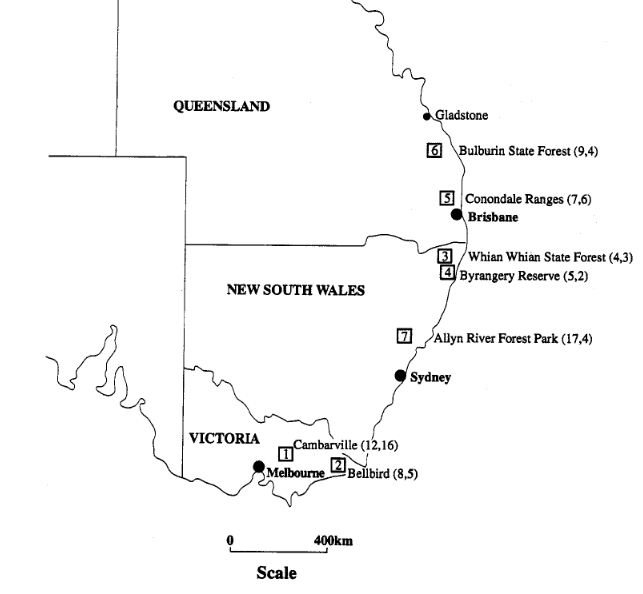
\includegraphics[width=0.7\linewidth]{../images/possum_age_plot} \end{center}

\begin{Shaded}
\begin{Highlighting}[]
\CommentTok{\# Preprocess data{-}set}
\end{Highlighting}
\end{Shaded}

\subsection{Feature Selection and Model
Training}\label{feature-selection-and-model-training}

\begin{Shaded}
\begin{Highlighting}[]
\CommentTok{\# Forward feature selection and model training}
\end{Highlighting}
\end{Shaded}

\subsection{Model Evaluation}\label{model-evaluation}

\begin{Shaded}
\begin{Highlighting}[]
\CommentTok{\# Compute evaluation metrics}
\end{Highlighting}
\end{Shaded}

\subsection{Further Exploration}\label{further-exploration}

\begin{Shaded}
\begin{Highlighting}[]
\CommentTok{\# Additional analysis or research questions}
\end{Highlighting}
\end{Shaded}


\end{document}
